\documentclass[conference]{IEEEtran}
\usepackage[utf8]{inputenc}
\usepackage{amsfonts}
\usepackage{caption}
\usepackage{graphicx}
\usepackage{listings}
\lstset{
    basicstyle=\tiny\ttfamily,
    keywordstyle=\color{blue}\ttfamily,
    stringstyle=\color{red}\ttfamily,
    commentstyle=\color{green}\ttfamily,
    breaklines=true
}
\usepackage{url}

% correct bad hyphenation here
\hyphenation{op-tical net-works semi-conduc-tor}

\begin{document}
\title{Relatório - EP2}

\author{\IEEEauthorblockN{Tiago Koji Castro Shibata - 8988730}
\IEEEauthorblockA{Escola Politécnica\\
Universidade de São Paulo\\
tiago.shibata@usp.br}
}

\maketitle

\section{Introdução}
Esse relatório acompanha o segundo exercício programa (EP2) da disciplina PCS3556 - Lógica Computacional.

\hfill 04 de Março de 2018

\section{Tarefa}

A tarefa consiste em implementar um algoritmo de reconhecimento de cadeias geradas por uma gramática de estrutura de frase recursiva. O algoritmo reconhecedor deve retornar se uma dada cadeia pode ser gerada por uma gramática.

\section{Algoritmo}

O algoritmo deve suportar qualquer gramática sensível ao contexto (ou seja, pela hierarquia de Chomsky, linguagens sensíveis ao contexto, livres de contexto e regulares são suportadas):
\\
\\
\begin{minipage}{\linewidth}
    \centering
    \label{chomsky}
    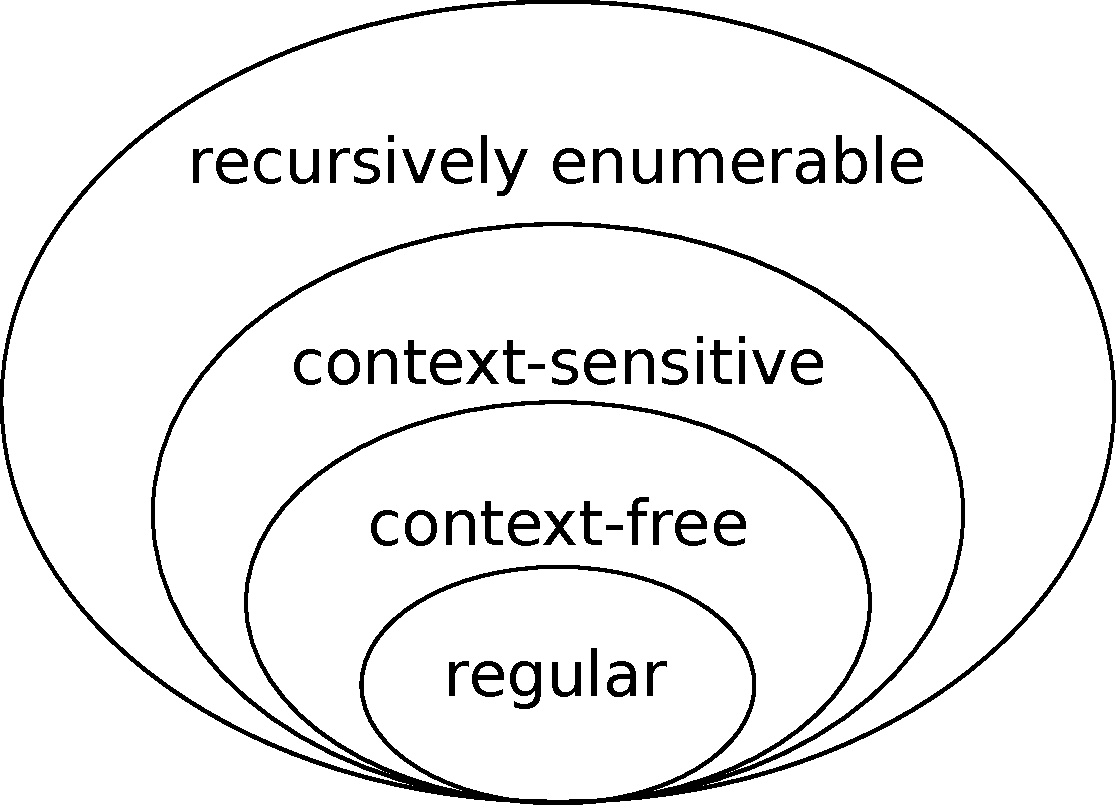
\includegraphics[width=0.8\textwidth]{Chomsky-hierarchy.pdf}
    \captionof{figure}{Hierarquia de Chomsky}
\end{minipage}

Conforme especifiado, a implementação é recursiva e feita em Elixir, uma linguagem funcional. Conforme sugerido no enunciado, foi implementada uma função de expansão a partir de uma forma sentencial inicial, gerando todas as formas sentenciais e sentenças intermediárias, e ao fim verificou-se a pretinência da sentença buscada na lista de sentenças geradas.

\section{Estruturas de dados}

Em alguns locais, estruturas de conjunto fornecidas pelo Elixir ($MapSet$) foram usadas tendo em mente performance e facilidade: o uso de conjunto evita que varramos a lista toda para buscar um elemento, e o conjunto permite operações fáceis e rápidas de união ou diferença quando necessário.

\section{Código e testes}

A função $apply\_rule(rule, state)$ recebe uma regra de substituição e um estado do gerador (uma sentença ou forma sentencial). Ela gera todas as formas sentenciais e sentenças possíveis aplicando essa regra no estado base.

A regra é dada como uma tupla $\{cadeia\ inicial, cadeia\ a\ ser\ colocada\}$. Foram escritos testes para essa função:

\lstinputlisting{1_test.ex}

Os testes foram essenciais no desenvolvimento, já que essa função apresenta muitos \emph{corner cases}. Por exemplo, casos com regras que batem em posições que se sobrepõe ($AA\ -> a$ com a forma sentencial AAA, por exemplo) falhariam em implementações básicas usando \emph{String.split} para buscar correspondências.

A função foi implementada buscando a primeira correspondência da condição da regra na forma sentencial com a função \emph{String.split}. Se não há correspondência, ocorre o fim da recursão. Se há, são feitas duas chamadas recursivas: uma realizando a substituição, que ira chamar $apply\_rule$ com o lado direito da cadeia, e outra não realizando a substituição, que avança um caractere da correspondência encontrada e chama $apply\_rule$:

\lstinputlisting{1.ex}

Depois, foram feitos testes e implementação de uma função que aplique uma lista de regras:

\lstinputlisting{2_test.ex}
\lstinputlisting{2.ex}

Então, foi feita uma função que aplica regras até um comprimento limite. Foram feitos testes com gramáticas livres de contexto, dependentes de contexto, e alguns \emph{corner cases}. Um caso notavelmente complicado foi regras que incluíssem expressões como $A\ -> B, B\ -> A$, já que há um ciclo entre A e B sem aumentar o tamanho da cadeia. A implementação deve acompanhar quais formas sentenciais já foram visitadas para não ficar presa em um ciclo no qual o comprimento se mantém.

\lstinputlisting{3_test.ex}

A implementação utiliza um $MapSet$ para acompanhar formas sentenciais geradas e outro para já visitadas. São feitas chamadas recursivas a $apply\_rules$ enquanto houver formas não visitadas.

\lstinputlisting{3.ex}

Algumas funções adicionais com interface mais simples foram definidas:

\lstinputlisting{4.ex}

E testes finais feitos:

\lstinputlisting{4_test.ex}

\begin{thebibliography}{1}
\bibitem{elixir}
Friedel Ziegelmayer. \emph{Elixir ExDoc}. \url{https://hexdocs.pm/elixir/}, acessado em 11/02/2018
\end{thebibliography}

\end{document}
